\documentclass[a4paper]{article} % TIPO DO DOCUMENTO
\usepackage[brazil]{babel} % Datas e nomes em Português com estilo Brasileiro
\usepackage[utf8]{inputenc} % Permite acentos
\usepackage{color} % Permite o uso de cores
\usepackage{graphicx} % permite o uso de figuras
\usepackage{fancyhdr}
\pagestyle{fancy}
%\usepackage{xcolor}  -- REMOVER
\usepackage{ulem}
\usepackage[pdftex]{hyperref}
\usepackage{wrapfig}
\usepackage{rotating}
%\usepackage{showframe}
\usepackage{marginnote}
\usepackage{caption}
\usepackage{xparse}
\usepackage{l3keys2e}
\usepackage{changepage}
\usepackage{scrextend}
\usepackage[marginparwidth=85pt]{geometry}
%\geometry{lmartin=3cm, tmartgin=3cm, rmargin=2,5cm,bmargin=1,75cm}
\usepackage[titletoc]{appendix}
\renewcommand{\appendixname}{Apêndice}
\renewcommand{\appendixtocname}{Apêndice}
%\renewcommand*\cftappendixname{\appendixname\enspace} %permite usar apêndices
\usepackage{makeidx}
\usepackage[table,xcdraw]{xcolor}
\usepackage{indentfirst}
\newcommand{\perito}{LEONEL CARLOS DIAS FERREIRA}
\newcommand{\processo}{1005733-67.2020.8.26.0053}
\newcommand{\classe}{Procedimento Comum Cível }
\newcommand{\assunto}{Anulação de Débito Fiscal}
\newcommand{\requerente}{SPS – Suprimentos para Siderurgia Ltda.}
\newcommand{\shortrequerente}{SPS }
\newcommand{\requerida}{Fazenda Pública do Estado de São Paulo}
\newcommand{\shortrequerida}{FESP }
\newcommand{\nomfls}{em fl. 98 }
\newcommand{\nomorigfls}{em mesma fls. }
\newcommand{\autornome}{SPS – Suprimentos para Siderurgia Ltda.}
\newcommand{\reunome}{Fazenda Pública do Estado de São Paulo}
\newcommand{\comarca}{5ª Vara da Fazenda Pública da Comarca da Capital/SP}
\newcommand{\CurriculoPerito}{http://www.tjsp.jus.br/auxiliaresjustica/auxiliarjustica/consultapublica/perfil/3946}
\newcommand{\autorpos}{Requerente}
\newcommand{\reupos}{Requerida }
\newcommand{\dataprot}{06/01/2022}

\newcommand{\txtmargem}{Este documento é cópia do original, assinado digitalmente por LEONEL CARLOS DIAS FERREIRA e Tribunal de Justica do Estado de Sao Paulo, protocolado em 06/01/2022 às 20:16 , sob o número WFPA22700030621
nº 1 SP 305.622/O-5 | CNPC/CFC nº 4.188 | CNAI/CFC nº 7.758
Para conferir o original, acesse o site https://esaj.tjsp.jus.br/pastadigital/pg/abrirConferenciaDocumento.do, informe o processo 1005733-67.2020.8.26.0053 e código C2A6D13.}


% Verificar para puxar um comando de outra 

%\usepackage[lmartin=3cm, tmartgin=3cm, rmargin=2,5cm,bmargin=1,75cm]{geometry}
%\usepackage{makeidx}
\usepackage{tabularx} %outro modo de fazer tabelas
\usepackage{array}
\setlength{\parindent}{4em} % Tamanho do parágrafo
\setlength{\parskip}{1.5em} % Espaço entre as linhas
\renewcommand{\baselinestretch}{1.5} % Espaço entre as linhas de um mesmo paragrafo
%\pagestyle{fancy}
\fontfamily{Arial narrow}
\fancyhf{} % limpa as configurações de rodapé e cabeçalho
\usepackage{lastpage} % permite usar a ultima pagina como referencia no rodapé
\usepackage{multicol}
%%
%% Cabeçalho
\lhead
{\begin{picture}(0,0)
\put(100,15) % Coordenadas do cabeçalho na página
{
\includegraphics[scale=1]{Imagens/cabecalho.png}}
\end{picture}}

\lfoot{
\begin{tabular}{l|r}
    Av. Regente Ferjó, 944 - Conj.1604-A & 
    \begin{picture}(0,0)
    %\put(100,0)
    
\includegraphics[scale=0.05]{Imagens/WhatsApp_Logo_sem fundo.png}
    \end{picture}(11) 9-3724-8706\\
    Anália Franco CEP: 03.342-000 - São Paulo/SP & lfpa@ifpa.com.br
     & 
\end{tabular}}



\rfoot{ 

\thepage \hspace{1pt} - \pageref{LastPage}
}



\begin{document}


\begingroup
%\setlength{\parindent}{4em} % Tamanho do parágrafo
\setlength{\parskip}{0.5em} % Espaço entre as linhas
\renewcommand{\baselinestretch}{0.5} % Espaço entre as linhas de um mesmo paragrafo
\textbf{MM.Juízo da \comarca }
\vspace{10cm} % Vspace adiciona um espaço vertical do tamanho informado

\begin{tabular}{r l}
    \textbf{Processo nº:} & \processo    \\
    \textbf{Classe:}     &   \classe     \\
    \textbf{Assunto:}    &   \assunto    \\
    \textbf{Requerentes:} &  \requerente \\
    \textbf{Executada:} & \requerida     \\
\end{tabular}\\


\textbf{LEONEL CARLOS DIAS FERREIRA}, Perito Contábil\footnote{\CurriculoPerito} inscrito no CRC/SP sob o nº 1 SP 305.622/O-5, CNPC/CFC nº 4.188 e CNAI/CFC nº 7.758, este honrosamente designado para realizar o exame pericial contábil conforme determinado \nomfls dos autos do processo em epígrafe, em atendimento aos termos estabelecidos em decisão proferida \nomorigfls dos autos do Procedimento Ordinário, vem mui respeitosamente à presença de V. Ex.ª apresentar o seu: \\
\begin{center}
    \huge \textbf{LAUDO PERICIAL CONTÁBIL} 
\end{center}

\endgroup
 
\tableofcontents
\listoffigures
\listoftables
\newpage

\section{Considerações Preliminares}
\input{1 - Considerações Preliminares/1.1 - Modelos-Resumo-da-Lide/Resumo da LIDE.txt}

\newpage
\input{1 - Considerações Preliminares/1.2 - Deferimento, objeto e objetivo de Perícia/Deferimento, objetivo e objetivo da Perícia.txt}

\newpage
\input{1 - Considerações Preliminares/1.3 - Modelos Procedimentos Periciais Adotados/Procedimentos periciais adotados.txt}

\newpage
\input{1 - Considerações Preliminares/1.4 - Modelos Cumprimento do Termo de Solicitação de Elementos/1.4 - Cumprimento do Termo de Solicitação de Elementos.txt}

\input{1 - Considerações Preliminares/1.4 - Modelos Cumprimento do Termo de Solicitação de Elementos/1.4.1 - Acerca do não atendimento do Termo de Solicitação de Elementos.txt}

\input{1 - Considerações Preliminares/1.4 - Modelos Cumprimento do Termo de Solicitação de Elementos/1.4.2 - Da análise dos documentos juntados aos autos do processo.txt}

\newpage
\textbf{\section{Aspectos técnicos e balizas teóricas}}
\textbf{\subsection{Declaração de Inconstitucionalidade: Afastamento da taxa de juros previstas na Lei Estadual de São Paulo nº 13.918/09}}
O debate entorno do afastamento da incidência da taxa de juros prevista na Lei Estadual de São Paulo nº 13.918/09 foi notável.

Com a redação conferida pela Lei sob exame, a Lei Estadual de São Paulo nº 6.374/89 passou a prevê a multa e os juros incidentes sobre o crédito tributário nos seguintes termos:

\textbf{Lei nº 6.374, de 01 de março de 1989}
\textbf{Artigo 96}.   O montante do imposto ou da multa, aplicada nos termos do artigo 85 desta lei, fica sujeito a juros de mora, que incidem:\\
(...)

\textbf{II} - relativamente à multa aplicada nos termos do artigo 85 desta lei, a partir do segundo mês subsequente ao da lavratura do auto de infração.

\textbf{§ 1º} \emph{A taxa de juros de mora será de 0,13 \%  (treze décimos por cento) ao dia.}

\textbf{§ 2º} O valor dos juros deve ser fixado e exigido na data do pagamento do débito fiscal, incluindo-se esse dia.

\textbf{§ 3º} Na hipótese de auto de infração, pode o regulamento dispor que a fixação do valor dos juros se faça em mais de um momento.

\textbf{§ 4º} Os juros de mora previstos no § 1º deste artigo, poderão ser reduzidos por ato do Secretário da Fazenda, observando-se como parâmetro as taxas médias pré-fixadas das operações de crédito com recursos livres divulgadas pelo Banco Central do Brasil.

\textbf{§ 5º} Em nenhuma hipótese a taxa de juros prevista neste artigo poderá ser inferior à taxa referencial do Sistema Especial de Liquidação e de Custódia - SELIC para títulos federais, acumulada mensalmente."

Conforme reproduzido acima, nos termos da Lei Estadual de São Paulo nº 13.918/09, o imposto e a multa que sobre ele incide, sujeitam-se a juros de mora com taxa à razão de 0,13\% a.d. (treze décimos por cento ao dia), calculados sobre os acréscimos moratórios e sobre os valores das penalidades.

Essa sistemática prevista na legislação do Estado de São Paulo fixa taxa de juros que supera a estipulada pela União e, mesmo que haja a competência legislativa concorrente entre os Estados e União (artigo 24, inciso I, da Constituição Federal), firmou-se o entendimento que a fixação por parte dos Estados-membro não poderá superar ao estipulado pela União. Ante o exposto, o Órgão Especial do Tributal de Justiça do Estado de São Paulo (TJSP), no Incidente de Inconstitucionalidade nº 0170909-61.2012.8.26.0000, estabeleceu a incidência da Taxa SELIC como índice a ser observado, em substituição ao estipulado na Lei Estadual em análise:

INCIDENTE DE INCONSTITUCIONALIDADE - Arts. 85 e 96 da Lei Estadual nº 6.374/89, com a redação dada pela Lei Estadual nº 13.918/09 - \textcolor{red}{\emph{Nova sistemática de composição dos juros da mora para os tributos e multas estaduais (englobando a correção monetária) que estabeleceu taxa de 0,13\% ao dia, podendo ser reduzida por ato do Secretário da Fazenda, resguardado o patamar mínimo da taxa SELIC}} - Juros moratórios e correção monetária dos créditos fiscais que são, desenganadamente, institutos de Direito Financeiro e/ou de Direito Tributário - Ambos os ramos do Direito que estão previstos em conjunto no art. 24, inciso I, da CF, em que se situa a competência concorrente da União, dos Estados e do DF - §§ 1º a 4º do referido preceito constitucional que trazem a disciplina normativa de correlação entre normas gerais e suplementares, pelos quais a União produz normas gerais sobre Direito Financeiro e Tributário, enquanto aos Estados e ao Distrito Federal compete suplementar, no âmbito do interesse local, aquelas normas - \emph{STF que, nessa linha, em oportunidades anteriores, firmou o entendimento de que os Estados-membros não podem fixar índices de correção monetária superiores aos fixados pela União para o mesmo fim (v. RE nº 183.907-4/SP e ADI nº 442} - CTN que, ao estabelecer normas gerais de Direito Tributário, com repercussão nas finanças públicas, impõe o cômputo de juros de mora ao crédito não integralmente pago no vencimento, anotando a incidência da taxa de 1\% ao mês, “se a lei não dispuser de modo diverso” - Lei voltada à regulamentação de modo diverso da taxa de juros no âmbito dos tributos federais que, destarte, também se insere no plano das normas gerais de Direito Tributário/Financeiro, balizando, no particular, a atuação legislativa dos Estados e do DF - \textcolor{red}{\emph{Padrão da taxa SELIC que veio a ser adotado para a recomposição dos créditos tributários da União a partir da edição da Lei nº 9.250/95, não podendo então ser extrapolado pelo legislador estadual - Taxa SELIC que, por sinal, já se presta a impedir que o contribuinte inadimplente possa ser beneficiado com vantagens na aplicação dos valores retidos em seu poder no mercado financeiro, bem como compensar o custo do dinheiro eventualmente captado pelo ente público para cumprir suas funções}} - \emph{Fixação originária de 0,13\% ao dia que, de outro lado, contraria a razoabilidade e a proporcionalidade, a caracterizar abuso de natureza confiscatória, não podendo o Poder Público em sede de tributação agir imoderadamente} - Possibilidade, contudo, de acolhimento parcial da arguição, para conferir interpretação conforme a Constituição, em consonância com o julgado precedente do Egrégio STF na ADI nº 442 - Legislação paulista questionada que pode ser considerada compatível com a CF, desde que a taxa de juros adotada (que na atualidade engloba a correção monetária), seja igual ou inferior à utilizada pela União para o mesmo fim - Tem lugar, portanto, a declaração de inconstitucionalidade da interpretação e aplicação que vêm sendo dada pelo Estado às normas em causa, sem alterá-las gramaticalmente, de modo que seu alcance valorativo fique adequado à Carta Magna (art. 24, inciso I e § 2º) - Procedência parcial da arguição. (Des. PAULO DIMAS MASCARETTI, j. 27/02/2013).
\[\]
Desta forma, ficou estabelecido os juros moratórios no percentual previsto pela Taxa SELIC, ante a não observância da taxa formada pela Lei Estadual de São Paulo nº 13.918/09.

\newpage
\hypertarget{3.1}{\section{Constatações e Análises Periciais}}
\subsection{Do valor exigido}
No que tange ao valor exigido na presente \textbf{Ação}, a \reupos juntou aos autos cópia do Procedimento Administrativo que enseja o AIIM de n° 4.037.656-4 lavrado em 26/02/2014 (fls. 180/349 dos autos), do qual a \textbf{Perícia} assim reproduz a seguir o Demonstrativo do Débito Fiscal:
\newline
\hypertarget{tab1}{}
\begin{table}[h!]
    \centering
    \resizebox{\textwidth}{!}{
    \begin{tabular}{|m{1cm}|m{2cm}|m{1.7cm}|m{1cm}|m{1.4cm}|m{1.7cm}|m{2cm}|m{1.4cm}|m{1.6cm}|m{1cm}|m{1.5cm}|}
        \hline
        Item do AIIM & Valor Original do Tributo (R\$) & Termo Inicial Juros	& Taxa Juros FESP (\%)	& Valor dos Juros (R\$) & Valor Básico Multa (R\$) & Termo Inicial – Multa & Taxa Juros FESP(\%) & Valor Básico Atualizado (R\$) & Multa (\%) & Valor Multa (R\$) \\ \hline
        
        1 &	138.240,00 & 31/10/2012 & 14,78 & 20.431,87 & 844.800,00 &  31/10/2012 & 14,78 & 969.661,44 & 50,00 & 484.830,72 \\ \hline
        
        Total & 138.240,00 & & & 20.431,87 & 844.800,00 & & & 969.661,44 & & 484.830,72 \\ \hline
    \end{tabular}}
    \caption{Anexo ao AIIM n° 4.037.656-4 de 26/02/2014 (fl. 182 dos autos)}
    \label{tab:my_label}
\end{table}

%TODO indentar texto inicio:
\textbf{Constatação:} Dos valores supracitados, observa-se que o principal de imposto remonta em de \emph{\textbf{R\$ 138.240,00}} que, sendo base de cálculo para incidência da \emph{\textbf{taxa de juros nos patamares de 14,78\%}} resulta em \emph{\textbf{R\$ 20.431,87}} a título de juros, enquanto o valor básico para cálculo da multa punitiva remonta em \emph{\textbf{R\$ 844.800,00}} que, no mesmo percentual de atualização aplicado, resulta em \emph{\textbf{R\$ 969.661,44}}, figurando como base de cálculo para aplicação de 50\%, resultando em \emph{\textbf{R\$ 484.830,72}} de multa punitiva imposta. Neste sentido, o cerne da questão, consoante alegações da \emph{\textbf{Requerente}} em inicial e seguintes, é pela irregularidade do percentual de \emph{\textbf{atualização de 14,78\%}} a título de percentual de juros e atualização do valor básico para incidência da multa.
%fim do texto a ser indentado

Válido destacar que, do que se depreende da análise do AIIM \textit{sub judice}, tem-se no Relato da Infração (fl. 31 dos autos) que o valor relativo ao principal do imposto no montante
de \emph{\textbf{R\$ 138.240,00}} refere-se ao aproveitamento indevido de crédito de ICMS decorrente da escrituração de documentos fiscais que não correspondem a entrada de mercadorias do estabelecimento ou aquisição de sua propriedade sendo que estes documentos fiscais não atendem às condições previstas no item 3 do § 1° do art. 59 do RICMS/2000.
O período autuado compreende as notas emitidas em outubro de 2012 pela empresa Anelka Metais Não Ferrosos Ltda., a qual teve sua inscrição estadual declarada nula com efeitos retroativos desde 03/08/2012, ou seja, abarcando o período em que a \textbf{Requerente} manteve relações comerciais e escriturou documentos tidos como inidôneos pela \textbf{FESP}.
%TODO \emph não está quebrando página

No entanto, restringindo-se ao juízo técnico pericial demandando na presente Ação, a qual \emph{\textbf{limita o escopo da prova para tão somente confirmação dos valores a título de correção e juros incididos sobre o principal do imposto e valores básicos de multa punitiva pela aplicação da taxa de 14,78\% em detrimento da Taxa SELIC}}, a \textbf{Perícia} não adentrará no mérito da questão quanto à análise da origem do principal e sua composição.

\newpage
\subsection{Da constituição das atualizações e juros do principal e multa punitiva}

Do que consta aos Autos, a \textbf{Perícia} identificou vasta documentação por parte da \textbf{Requerida} no que se refere ao Procedimento Administrativo (fls. 180/349 dos autos) impetrado e que fundamenta do AIIM \textit{sub judice}, corroborando com a composição do débito exigido, conforme referenciado no \hyperlink{1.4.2}{\emph{Subtópico 1.4.2 - Da análise dos documentos juntados aos autos do processo}} retro, a \textbf{Perícia} avaliou os dados disponíveis no intuito de ratificá-los.


\newpage
\hypertarget{3.3}{\subsection{Das Taxas de Juros e Correção Aplicadas em cotejo com a Taxa SELIC}}

Conforme constatado no tópico anterior, a \textbf{FESP} aplicou na data da lavratura do AIIM de n° 4.037.656-4 taxas nos patamares de \textbf{14,78\%}, tanto para cálculo dos juros sobre o principal como para a atualização do valor básico para cálculo da multa punitiva, sendo esta a controvérsia que origina o exame pericial no caso em tela, uma vez que se alega na exordial que referida taxa supera os patamares da Taxa SELIC.

Neste diapasão, eximindo-se de quaisquer juízos de valor quanto à aplicabilidade ou não da Taxa SELIC em substituição às taxas adotadas pela \textbf{Requerida}, sendo esta atribuída oportunamente ao Juízo, a \textbf{Perícia} perseguiu na própria fonte de cálculo dos débitos tributários administrados pela União, qual seja o sítio da Receita Federal do Brasil, obtendo o que segue:

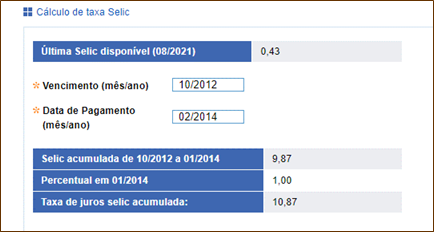
\includegraphics{Imagens/Figura 1 Taxa SELIC acumulada extraída do SICALC (Programa de Atualização Débitos da RFB).png}
%indentar texto abaixo:

\textbf{Constatação:} Constata-se que, considerando o termo inicial em outubro de 2012 (mês de competência das transações autuadas) e o mês da lavratura do AIIM (fevereiro de 2014), a Taxa SELIC Acumulada nos moldes estabelecidos pela União para os juros e correção dos débitos tributários perfaz \textbf{10,87\%} na data da lavratura do AIIM.
%Fim da indentação

Dessa forma, para fins de comparação entre o cálculo original do AIIM \textit{sub judice} (pautado na Lei Estadual nº 13.918/2009) e a tese da \textbf{Requerente} que requer limitação dos juros e correção aos patamares da Taxa SELIC (Arguição de Inconstitucionalidade nº 0170909-61.212.8.26.000), a Perícia substituiu o \textbf{percentual de 14,78\% (originário) por 10,87\% (Taxa SELIC acumulada conforme Receita Federal do Brasil)}, vejamos:

\begin{table}[h!]
    \centering
    \resizebox{\textwidth}{!}{
    \begin{tabular}{|m{1cm}|m{2cm}|m{1.7cm}|m{1cm}|m{1.4cm}|m{1.7cm}|m{2cm}|m{1.cm}|m{1.6cm}|m{1cm}|m{1cm}|m{2cm}|}
        \hline
        Item do AIIM & Valor Original do Tributo (R\$) & Termo Inicial Juros & Taxa Juros SELIC (\%) & Valor dos Juros (R\$) & Valor Básico Multa (R\$) & Termo Inicial – Multa & Taxa (\%) & Valor Básico Atualizado (R\$) & Multa (\%) & Valor Multa (R\$) \\ \hline
        
        1 &	138.240,00 & 31/10/2012 & 10,87 & 15.026,69 & 844.800,00 &  31/10/2012 & 10,87 & 936.629,76 & 50,00 & 468.314,88 \\ \hline
        
        Total & 138.240,00 & & & 15.026,69 & 844.800,00 & & & 936.629,76 & & 468.314,88 \\ \hline
    \end{tabular}}
    \caption{Recálculo do Anexo ao AIIM n° 4.037.656-4 em 26/02/2014}
    \label{tab:my_label}
\end{table}

%Texto a ser indentado
\textbf{Constatação:} Constata-se que, aplicando a taxa de \textbf{10,87\%} identificada no próprio programa que acumula a Taxa SELIC e que remunera os débitos federais (tese da \textbf{Requerente)}, o resultado de juros perfaz o montante de \textbf{R\$ 15.026,69} enquanto o valor básico da multa punitiva atualizado em fevereiro de 2014 resulta no montante de
\textbf{R\$ 936.629,76}, figurando como base de cálculo para aplicabilidade da multa calculada em \textbf{R\$ 468.314,88}.
%fim da indentação

Dessa forma, visando ilustrar a comparação entre os valores resultantes do AIIM originário e aqueles calculados pela \textbf{Perícia} consoante tese da Requerente, vejamos a tabela a seguir:

\hypertarget{tab3}{}
\begin{table}[h!]
    \centering
    %\resizebox{\textwidth}{!}{
    \begin{tabular}{|m{2cm}|m{2cm}|m{1.7cm}|m{1.5cm}|}
        \hline
        Origem & Valor dos Juros (R\$) & Valor da Multa (R\$) & Diferença Total (R\$) \\ \hline
        
        AIIM Original & 20.431,87 & 484.830,72 & \\ \hline
        
        AIIM Recálculo & 15.026,69 & 468.314,88 & \\ \hline
        
        DIFERENÇA & 5.405,18 & 16.515,84 & 21.921,02 \\ \hline
    \end{tabular}
    %}
    \caption{Resumo da comparação entre Juros e Multa do AIIM Original em cotejo com o Recálculo (Taxa SELIC)}
    \label{tab:my_label}
\end{table}

%Texto a ser indentado
\textbf{Constatação:} Constata-se que, entre o cálculo do AIIM originário e o recálculo da \textbf{Perícia}, apura-se uma diferença de juros exigidos a maior da \textbf{Requerente} em \textbf{R\$ 5.405,18}, da mesma forma apurando-se a diferença a maior de \textbf{R\$ 16.515,84} a título de multa punitiva, totalizando uma diferença de \textbf{R\$ 21.921,02} na data-base 26/02/2014 (data da lavratura).
% Fim do texto a ser indentado

Portanto, conclui-se que \emph{o percentual de 14,78\% adotado como taxa juros} aplicada sobre o principal do imposto e adotada para correção do valor básico (base de cálculo) da multa punitiva \emph{é superior aos patamares da Taxa SELIC que, para o mesmo período de lavratura do AIIM, resulta em 10,87\%} consoante parâmetros estabelecidos pela Receita Federal do Brasil (União), nos termos da Arguição de Inconstitucionalidade nº 0170909-61.212.8.26.000, ofertando à V. Exa. o resultado deste e ficando este \textbf{signatário} à disposição para as atualizações que julgar necessárias.

\newpage
\section{Considerações Finais}
O Laudo Pericial Contábil foi estruturado a partir de bases provenientes das normas contábeis disseminadas pelo Conselho Federal de Contabilidade (CFC), as práticas contábeis, os conceitos da matemática financeira atinentes e atendimento às normas relativas à elaboração e apresentação de elementos consignados pela Associação Brasileira de Normas Técnicas (ABNT).

Trata-se de Ação Ordinária com Pedido de Antecipação dos Efeitos da Tutela ajuizada por \textbf{\requerente} em face da \textbf{\requerida}, distribuídos sob o número \textbf{\processo}

Em relação ao quanto \textit{debeatur}, o trabalho pericial examinou os documentos juntados aos autos, em especial o AIIM 4.037.656-4 lavrado em vinte e seis de fevereiro de 2014,
originando a CDA n° 1.206.810.346 de janeiro de 2016.

Restringindo-se ao objeto da demanda, qual seja da constatação da aplicabilidade de taxa de juros e de correção especificadas no AIIM em detrimento da limitação aos patamares da Taxa SELIC, consoante julgamento da Arguição de Inconstitucionalidade nº 0170909-61.2012.8.26.000, a \textbf{Perícia} passou a obter, para que não reste dúvidas, no próprio sítio da Receita Federal do Brasil a Taxa SELIC para época da lavratura do AIIM \textit{sub judice}, constatando:
%TODO texto a ser indentado:

\textbf{(i)} Do AIIM 4.037.656-4 (fls. 180/183 dos autos), constatou-se que o principal de imposto remonta em \textbf{R\$ 138.240,00} que, sendo base de cálculo para \textit{incidência da taxa de juros nos patamares de 14,78\%} resulta em \textbf{R\$ 20.431,87} a título de juros, enquanto que, o valor básico para cálculo da multa punitiva remonta em \textbf{R\$ 844.800,00} que, no mesmo percentual de atualização aplicado \textbf{(14,78\%)}, resulta em \textbf{R\$ 969.661,44}, figurando como base de cálculo para aplicação de 50\% (percentual da penalidade), resultando em \textbf{R\$ 484.830,72} de multa punitiva aplicada, valores à época da lavratura em 26/02/2014.

\textbf{(ii)} A \textbf{Perícia} perseguiu a Taxa SELIC considerando os parâmetros de termo inicial (outubro de 2012) e data da lavratura do AIIM sub judice (fevereiro de 2014), na própria fonte de cálculo dos débitos tributários administrados pela União (sítio da Receita Federal do Brasil), constatando que, \textit{a Taxa SELIC Acumulada perfaz \textbf{10,87\%} considerando a data da lavratura do AIIM}.

\textbf{(iii)} Dessa forma, aplicando a taxa de \textbf{10,87\%} identificada no próprio programa que acumula a Taxa SELIC e que remunera os débitos federais (tese da Requerente), o resultado de juros perfaz o montante de \textbf{R\$ 15.026,69} sobre o principal, enquanto o valor básico da multa punitiva resulta no montante de \textbf{R\$ 936.629,76}, figurando como base de cálculo para aplicabilidade da multa calculada em \textbf{R\$ 468.314,88}.

\textbf{(iv)} Desta feita, a \hyperlink{tab3}{\emph{Tabela 3: Comparação entre Juros e Multa do AIIM Original vs Recálculo (Taxa SELIC)}} do \hyperlink{3.3}{\emph{Subtópico 3.3 - Das Taxas de Juros e Correção Aplicadas vs Taxa SELIC}} apresenta uma diferença total de \textbf{R\$ 21.921,02} (somatório dos juros exigidos a maior da \textbf{Requerente} em \textbf{R\$ 5.405,18} com a diferença a maior de \textbf{R\$ 16.515,84} a título de multa punitiva), em virtude da aplicação da taxa de \textbf{14,78\%} em detrimento dos limites da Taxa SELIC acumulada, a qual resultou em \textbf{10,87\%} para o mesmo período.

\newpage
\section{Encerramento}

Assim, encerra-se o presente \textbf{Laudo Pericial Contábil}, emitido em \textbf{33 (trinta e três) páginas}, processados eletronicamente e estando a última página assinada e datada.

Acompanha a presente peça os seguintes \textbf{Apêndices} e \textbf{Anexos}:

\textbf{Apêndices}:

\hyperlink{apA}{\emph{Apêndice A:	Respostas aos Quesitos da Requerente}} e

\hyperlink{ApB}{\emph{Apêndice B:	Respostas aos Quesitos da Requerida}}


Aproveita-se o ensejo para agradecer a nobre oportunidade de ter servido V. Exa. nos aspectos contábeis aplicadas à matéria, se colocando à disposição para os esclarecimentos que se fizerem necessários, bem como para novos trabalhos.


Nesses termos em que, respeitosamente, pede e espera deferimento.

\centering

São Paulo, \dataprot


\includegraphics[]{Imagens/Assinatura Leonel.png}\\
\textbf{Leonel Carlos Dias Ferreira}\\
CRC nº 1 SP 305.622/O-5 | CNPC/CFC nº 4.188 | CNAI/CFC nº 7.758

\newpage
\appendix
\addappheadtotoc % Adiciona o Título Apêndice
\flushleft
\hypertarget{apA}{\section{Quesitos formulados pela Requerente}}

\begin{enumerate}
    \item \textbf{Com relação à base de cálculo da multa punitiva:}

\textbf{Qual foi o índice utilizado pela FESP para obtenção do “Valor Básico Atualizado” da multa (colunas 8 e 9 do demonstrativo do débito fiscal acostado às fls. 33)?} \\
Resposta:	O índice adotado pela \textbf{\shortrequerida}para obtenção do “Valor Básico Atualizado” da multa, representado pelo montante de \textbf{R\$ 969.661,44}, foi de \textbf{14,78\%} (coluna 8) incidente sobre o valor básico de \textbf{R\$ 844.800,00} (coluna 6) do Demonstrativo do Débito Fiscal à fl. 33 dos autos.

\textbf{Qual foi a Taxa SELIC acumulada neste mesmo período?}

\textbf{Resposta:} Conforme minuciosamente explanado no \hyperlink{3.3}{Subtópico 3.3 - Das Taxas de Juros e Correção Aplicadas vs Taxa SELIC} deste Laudo Pericial Contábil, a \textbf{Perícia} perseguiu a Taxa SELIC considerando os parâmetros de termo inicial (outubro de 2012) e data da lavratura do AIIM \textit{sub judice} (fevereiro de 2014),
na própria fonte de cálculo dos débitos tributários administrados pela União (sítio da Receita Federal do Brasil), constatando que, a \textbf{Taxa SELIC acumulada} perfaz, em verdade, \textbf{10,87\%} na data da lavratura do AIIM.

\textbf{Podemos afirmar que os percentuais aplicados pela \shortrequerida para obtenção do “Valor Básico Atualizado” são superiores à Taxa SELIC?}

\textbf{Resposta:} Positiva é a resposta, em virtude da aplicação da taxa de \textbf{14,78\%} em detrimento dos limites da Taxa SELIC Acumulada, a qual resultou em \textbf{10,87\%} para o mesmo período.

\textbf{Podemos afirmar que ao aplicarmos a Taxa SELIC para obtenção do “Valor Básico Atualizado” da multa o valor final efetivamente devido pela Autora a título de multa punitiva será reduzido?}
\textbf{Resposta:} Positiva é a resposta. Aplicando-se a taxa de \textbf{10,87\%} identificada no próprio programa que acumula a Taxa SELIC e que remunera os débitos federais (tese da \textbf{Requerente)}, o valor básico da multa punitiva resulta no montante de \textbf{R\$ 936.629,76}, figurando como base de cálculo para aplicabilidade da multa calculada em \textbf{R\$ 468.314,88} sendo inferior ao montante calculado originalmente no AIIM sub judice, qual seja de \textbf{R\$ 484.830,72} para o mesmo período.

    \item \textbf{Com relação aos juros de mora do principal:}
\textbf{Qual foi o índice utilizado pela FESP para cálculo dos juros de mora do principal?}
\textbf{Resposta:} O índice adotado pela \textbf{\shortrequerida} para cálculo dos juros de mora do principal foi de \textbf{14,78\%} (coluna 4) incidente sobre o valor principal de \textbf{R\$ 138.240,00} (coluna 2), resultando no montante de \textbf{R\$ 20.431,87} (coluna 5) de juros evidenciado no Demonstrativo do Débito Fiscal à fl. 33 dos autos na data da lavratura.

\textbf{Qual foi a Taxa SELIC acumulada neste mesmo período?}

\textbf{Resposta:}	Conforme minuciosamente explanado no \hiperlink{3.3}{Subtópico 3.3 – Das Taxas de Juros e Correção Aplicadas em cotejo com a Taxa SELIC} deste Laudo Pericial Contábil, a \textbf{Perícia} perseguiu a Taxa SELIC considerando os parâmetros de termo inicial (outubro de 2012) e data da lavratura do AIIM \textit{sub judice} (fevereiro de 2014), na própria fonte de cálculo dos débitos tributários administrados pela União (sítio da Receita Federal do Brasil), constatando que, a Taxa SELIC acumulada perfaz \textbf{10,87\%} na data da lavratura do AIIM. 

\textbf{Podemos afirmar que os percentuais aplicados pela \shortrequerida para cálculo dos juros de mora do principal são superiores à Taxa SELIC?}
\textbf{Resposta:}	Positiva é a resposta, em virtude da aplicação da taxa de \textbf{14,78\%} em detrimento dos limites da Taxa SELIC Acumulada, a qual resultou em \textbf{10,87\%} para o mesmo período.

\textbf{Podemos afirmar que ao aplicarmos a Taxa SELIC para cálculo dos juros de mora do principal o valor final efetivamente devido pela Autora a título de juros de mora do principal será reduzido?}
\textbf{Resposta:}	Positiva é a resposta, aplicando a taxa de 10,87\% identificada no próprio programa que acumula a Taxa SELIC e que remunera os débitos federais (tese da \textbf{Requerente}), o resultado dos juros de mora perfaz o montante de \textbf{R\$ 15.026,69}, sendo inferior ao montante calculado originalmente no AIIM \textit{sub judice}, qual seja, de \textbf{R\$ 20.431,87} para o mesmo período.

    \item \textbf{Com relação aos juros de mora da multa:}
\textbf{Qual foi o índice utilizado pela FESP para cálculo dos juros de mora do principal?}
\textbf{Resposta:} Considerando a referência do quesito, compreende a Perícia que se trata de análise da CDA de n° \textbf{1.206.810.346} na qual é o único documento acostado aos autos que se visualiza os juros de mora incidentes sobre a multa punitiva.
\end{enumerate}
Neste sentido, vejamos a reprodução da CDA acostada à fl. 349 dos autos:

\begin{figure}
    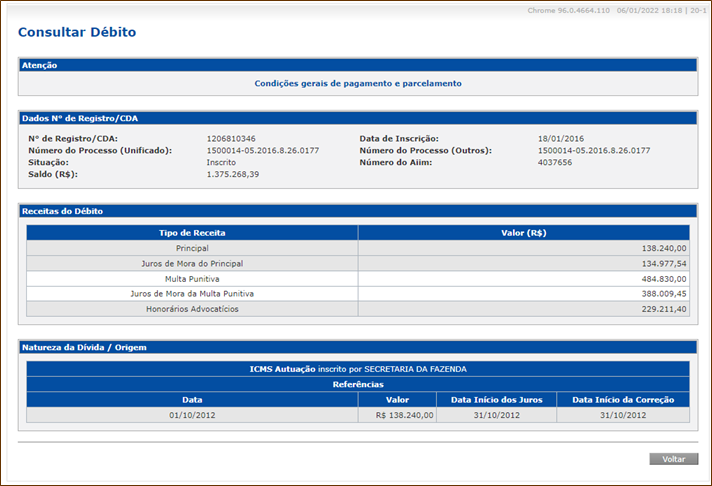
\includegraphics[width=1\textwidth]{Imagens/CDA n 1206810346 acostada a fl. 349 dos autos.png}
    \caption{CDA n° 1206810346 acostada à fl. 349 dos autos (emitida em 06/01/2021)}
    \label{fig:my_label}
\end{figure}


\begin{addmargin}[6cm]{} % Adiciona margim de recuo no texto

É possível observar que, a CDA supracitada foi emitida com posição de 06/08/2021, considerando que, nesta data, o valor de juros de mora da multa punitiva remonta em R\$ 388.009,45 sobre o valor principal da multa de R\$ 484.830,00, ou seja, depreende-se que o percentual de juros aplicado é de 80,04\%.
    \begin{itemize}
        \item \textbf{Qual foi a Taxa SELIC acumulada neste mesmo período?}

    \textbf{Resposta:} Considerando que se trata de novo posicionamento temporal de comparação, a \textbf{Perícia} perseguiu a Taxa SELIC acumulada considerando os parâmetros de termo inicial (outubro de 2012) e data do posicionamento da CDA de fl. 349 (agosto de 2021), na própria fonte de cálculo dos débitos tributários administrados pela União (sítio da Receita Federal do Brasil ), constatando que, a Taxa SELIC acumulada perfaz \textbf{74,79\%} para o mesmo período, vejamos:

\begin{figure}[!h]
    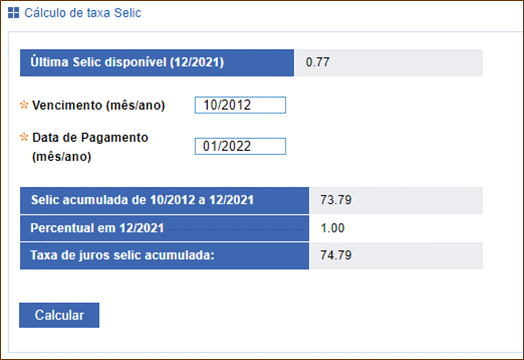
\includegraphics{Imagens/Taxa SELIC acumulada extraída do SICALC (Programa de Atualização Débitos da RFB).png}
    \caption{Taxa SELIC acumulada extraída do SICALC (Programa de Atualização Débitos da RFB)}
    \label{fig:my_label}
\end{figure}

%\newgeometry{left = 8cm} %muda a margem esquerda para 5cm
 \item \textbf{Podemos afirmar que os percentuais aplicados pela FESP para cálculo dos juros de mora da multa punitiva são superiores à Taxa SELIC?}
\textbf{Resposta:} Positiva é a resposta. Em virtude da aplicação da taxa de \textbf{80,04\%} em detrimento dos limites da Taxa SELIC acumulada, a qual resultou em \textbf{74,79\%} para o mesmo período.

\item \textbf{Podemos afirmar que ao aplicarmos a Taxa SELIC para cálculo dos juros de mora da multa punitiva o valor final efetivamente devido pela Autora a título de juros de mora da multa punitiva será reduzido?}

\textbf{Resposta:} Positiva é a resposta, aplicando a taxa de \textbf{74,79\%} identificada no próprio programa que acumula a Taxa SELIC e que remunera os débitos federais (tese da \textbf{Requerente}), o resultado dos juros de mora da multa punitiva perfaz o montante de \textbf{R\$ 350.252,70} já considerando que o percentual de \textbf{74,79\%} seja aplicado sobre a multa punitiva recalculada no valor de \textbf{R\$ 468.314,88}, sendo inferior ao montante calculado originalmente na CDA de fl. 349 dos autos, em referência ao quanto perquirido no quesito.
%\newgeometry{left = 3cm}
\end{itemize}
\end{addmargin}


\hypertarget{ApB}{
\section{Apêndice A: Respostas aos Quesitos da Requerente}}

\textbf{1.	Queira o I. Perito Judicial transcrever na integra os itens destacados no “Relato da Infração do documento 1 (fls.31/34), AIIM nº 4.037.656, destacando o montante das operações que infringiram o RICMS, e serviram como base para multa punitiva;}

\textbf{Resposta:} Visando prover celeridade e economicidade processual, respeitosamente, a \textbf{Perícia} pede reporte ao AIIM n° \textbf{4.037.656-4} acostado na íntegra às fls. 180/183 dos autos, para visualização do quanto perquirido no atual quesito.

\textbf{2.	Queira o I. Perito Judicial informar, conforme os documentos acostados nos autos, se Agente Fiscal atuante observou integralmente e relatou, os registros contábeis da Autora para fundamentar a lavratura do mencionado Auto de infração e imposição de Multa que originou a Certidão de Dívida Ativa ora executada.}

\textbf{Resposta:} Esclarece este signatário que, conforma explanado no item \textbf{“1.2 Deferimento, objeto e objetivo da Perícia”} do Laudo Pericial Contábil, restringindo-se ao juízo técnico pericial demandando na presente Ação, a \textbf{Perícia} limita o escopo da prova para tão somente confirmação dos valores a título de correção e juros incididos sobre o principal do imposto e valores básicos de multa punitiva pela aplicação da taxa de \emph{14,78\%} adotada na data da lavratura do AIIM em detrimento da Taxa SELIC, não adentrando, portanto, no mérito da questão quando a análise da origem do principal e sua composição, motivo pelo qual, prejudicada a resposta.

\textbf{3.	Queira o I. Perito Judicial informar, qual a penalidade por creditar-se indevidamente do ICMS, com fundamento no item 3 do §1º do artigo 59 do RICMS/2000. INFRINGÊNCIA: Arts. 59, §1°, item 3, arts. 61, art. 64, Inc. I, do RICMS (Dec.45.490/00)}

\textbf{Resposta:} Visando prover celeridade e economicidade processual, respeitosamente, a Perícia pede reporte a resposta ao quesito imediatamente anterior.

\textbf{4.	Queira o I. Perito Judicial demonstrar, se houve observação no documento 1 (fls.31/34), AIIM nº 4.037.656, e quais os termos e condições do Artigo 95, incisos I e II e §§ 1º e 8º, da Lei 6.374/89, na redação dada pela Lei 13.918/09, de 22/12/2009, para a multa e, nos termos do artigo 100 do Decreto nº 54.486/2009, sobre prazo para a defesa;}

\textbf{Resposta:} Atendendo ao quanto perquirido, a \textbf{Perícia} confirma que as referências de legislação sugerida no quesito estão contempladas no AIIM \textit{sub judice} (fls. 31/34 dos autos), de modo que, reproduz a capitulação legal no que concerne as penalidades aplicadas, uma vez que está contemplado no objeto da demanda, vejamos:

\textbf{Artigo 95 Inciso I e II e § 1° e 8° da Lei 6.374/89, redação dada pela Lei 13.918/09}

“(...)

Artigo 95 - Pode o autuado pagar a multa aplicada nos termos do artigo 85 desta lei, com desconto de: (NR)

I - 70\% (setenta por cento), dentro do prazo de 15 (quinze) dias contados da notificação da lavratura do auto de infração; (NR)

II - 60\% (sessenta por cento), dentro do prazo de 30 (trinta) dias contados da notificação da lavratura do auto de infração; (NR)

(...)

§ 1º - Condiciona-se o benefício ao integral pagamento do débito. (NR)

(...)

§ 8º – Tratando-se de penalidade aplicada sobre o valor do imposto, a aplicação dos descontos previstos neste artigo não poderá resultar em penalidade inferior a 25\% (vinte e cinco por cento) do valor do imposto. (NR)

(...)

Artigo 100 do Decreto n° 54.486/2009

(...) 

\textbf{Artigo 100} - Lavrado o auto de infração, terão início os procedimentos de cobrança administrativa, devendo o autuado ser notificado a recolher o débito fiscal, com o desconto de lei, quando houver, ou a apresentar defesa, por escrito, no prazo de 30 (trinta) dias.
§ 1º - Decorrido o prazo previsto no “caput” deste artigo sem que haja o recolhimento ou acordo de parcelamento do débito fiscal ou a apresentação de defesa, o auto de infração será encaminhado à Delegacia Regional Tributária da circunscrição do autuado para a sua ratificação pelo Delegado Regional Tributário.
§ 2º - Após a ratificação do auto de infração, e encerrados os procedimentos de cobrança administrativa sem o devido recolhimento ou acordo de parcelamento, o débito fiscal será inscrito na dívida ativa.
§ 3º - Em caso de apresentação de defesa parcial, e não sendo recolhido ou parcelado o débito fiscal correspondente à exigência não impugnada, o órgão de julgamento providenciará a formação de processo em apartado para os fins previstos nos parágrafos anteriores, consignando-se essa circunstância mediante termo no processo original e prosseguindo-se no julgamento quanto às exigências impugnadas.
§ 4º - Considera-se parcial a defesa na qual o interessado não conteste, de forma expressa, um ou mais itens de acusação.

(...)

\textbf{5.	Queira o I. Perito Judicial demonstrar, a composição de cálculo dos valores apresentados no documento 1 (fls.31/34), e em comparação as fundamentações legais por “infringência” e “Capitulação da Multa”, responder se os mesmos cálculos correspondem corretamente com o apurado.:}

\textbf{Resposta:}	Conforme amplamente explanado no \hyperlink{3.1}{Subtópico 3.1 - Do valor exigido} do Laudo Pericial Contábil, a \hyperlink{tab1}{Tabela 1: Anexo ao AIIM n° 4.037.656-4 de 26/02/2014 (fl. 182 dos autos)} evidencia a evolução do cálculo impetrado no AIIM \textit{sub judice}, mais precisamente pela reprodução do Demonstrativo do Débito Fiscal, no qual se pode constatar que, o principal de imposto remonta em \textbf{R\$ 138.240,00} que, sendo base de cálculo para incidência da \textbf{taxa de juros nos patamares de 14,78\%} resulta em \textbf{R\$ 20.431,87} a título de juros, enquanto que, o valor básico para cálculo da multa punitiva remonta em \textbf{R\$ 844.800,00} que, no mesmo percentual de atualização aplicado, resulta em \textbf{R\$ 969.661,44}, figurando como base de cálculo para aplicação de 50\%, resultando em \textbf{R\$ 484.830,72} de multa punitiva imposta.
No que se refere a comparação com a capitulação legal, ressalva a \textbf{Perícia} que a “infringência” e “capitulação da multa”, não se configuram matéria a ser apreciada no objeto da prova pericial perquirida, mas sim, tão somente as taxas incididas sobre o principal (figurando os juros) e sobre o valor básico (figurando correção) para aplicação do percentual de multa de 50\%, do qual não se discute nesta fase processual.

\textbf{6.	Queira o I. Perito Judicial informar, se a coluna 9 do cálculo de fl. 33, demonstra a correta aplicação do §9º do art. 85 da lei 6.374/89?}

\textbf{Resposta:}	Considerando a referência sugerida no quesito, a coluna 9 do cálculo de fl. 33 dos autos é resultando da aplicação da taxa de 14,78\% (coluna 8) sobre o valor básico de R\$ 844.800,00 (coluna 6) resultando assim no importe de R\$ 969.661,44, (coluna 9), sendo que, assim tem-se a capitulação legal do §9º do art. 85 da Lei 6.374/89:

(...)

§ 9º - As multas previstas neste artigo, excetuadas as expressas em UFESP, devem ser calculadas sobre os respectivos valores básicos atualizados observando-se o disposto no artigo 96 desta lei; (NR)

(...)

Artigo \textbf{96} da Lei 6.374/89

(...)

Artigo 96 - O montante do imposto ou da multa, aplicada nos termos do artigo 85 desta lei, fica sujeito a juros de mora, que incidem: (NR)
I - relativamente ao imposto: (NR)
a) a partir do dia seguinte ao do vencimento, caso se trate de imposto declarado ou transcrito pelo fisco nos termos dos artigos 56 e 58 desta lei, de parcela devida por contribuinte enquadrado no regime de estimativa e de imposto exigido em auto de infração, nas hipóteses das alíneas “b”, “c”, “d”, “e”, “f”, “g”, “h”, “i”, “j” e “l” do inciso I do artigo 85 desta lei; (NR)
b) a partir do dia seguinte ao último do período abrangido pelo levantamento, caso se trate de imposto exigido em auto de infração na hipótese da alínea “a” do inciso I do artigo 85 desta lei; (NR)
c) a partir do mês em que, desconsiderada a importância creditada, o saldo tornar-se devedor, caso se trate de imposto exigido em auto de infração, nas hipóteses das alíneas “b”, “c”, “d”, “h”, “i” e “j” do inciso II do artigo 85 desta lei; (NR)
d) a partir do dia seguinte àquele em que ocorra a falta de pagamento, nas demais hipóteses; (NR)
II - relativamente à multa aplicada nos termos do artigo 85 desta lei, a partir do segundo mês subsequente ao da notificação da lavratura do auto de infração. (NR)
§ 1º - A taxa de juros de mora é equivalente: (NR) 
1 - por mês, à taxa referencial do Sistema Especial de Liquidação e de Custódia - SELIC para títulos federais, acumulada mensalmente; (NR)
2 - a 1\% (um por cento) para fração de mês, assim entendido qualquer período de tempo inferior a um mês; (NR)
§ 2º - Ocorrendo a extinção, substituição ou modificação da taxa prevista no item 1 do § 1º, o Poder Executivo adotará outro indicador oficial que reflita o custo do crédito no mercado financeiro. (NR)
§ 3º - O valor dos juros deve ser fixado e exigido na data do pagamento do débito fiscal, incluindo-se esse dia. (NR)
§ 4º - Na hipótese de auto de infração, pode o regulamento dispor que a fixação do valor dos juros se faça em mais de um momento. (NR)
§ 5º - A Secretaria da Fazenda divulgará, mensalmente, a taxa a que se refere este artigo. (NR)

(...)

Objetivamente, conclui-se que o percentual de 14,78\% adotado como taxa juros aplicados sobre o principal do imposto e adotada para correção do valor básico (base de cálculo) da multa punitiva é, fatidicamente, superior aos patamares da Taxa SELIC que, para o mesmo período de lavratura do AIIM, resulta em 10,87\% consoante parâmetros estabelecidos pela Receita Federal do Brasil - União.

\textbf{7.	Queira o I. Perito Judicial, demonstrar qual valor apurou em seus cálculos como montante principal, juros e multa punitiva à época e demonstrá-las:}

\textbf{Resposta:}	Conforme minuciosamente explanado no \hyperlink{3.3}{\emph{Subtópico 3.3 – Das Taxas de Juros e Correção Aplicadas em cotejo com a Taxa SELIC}} deste Laudo Pericial Contábil, a \textbf{Perícia} perseguiu a Taxa SELIC considerando os parâmetros de termo inicial (outubro de 2012) e data da lavratura do AIIM \textit{sub judice} (fevereiro de 2014), na própria fonte de cálculo dos débitos tributários administrados pela União (sítio da Receita Federal do Brasil), constatando que, a Taxa SELIC acumulada perfaz \textbf{10,87\%} na data da lavratura do AIIM.

Dessa forma, aplicando a taxa de \textbf{10,87\%} identificada no próprio programa que acumula a Taxa SELIC e que remunera os débitos federais (tese da \textbf{Requerente}), o resultado de juros perfaz o montante de \textbf{R\$ 15.026,69} sobre o principal, enquanto o valor básico da multa punitiva resulta no montante de \textbf{R\$ 936.629,76}, figurando como base de cálculo para aplicabilidade da multa calculada em \textbf{R\$ 468.314,88.}

Assim, apurou-se uma diferença total de \textbf{R\$ 21.921,02}
(somatório dos juros exigidos a maior da \textbf{Requerente} em
\textbf{R\$ 5.405,18} apurando-se, da mesma forma, a diferença a maior de \textbf{R\$ 16.515,84} de multa punitiva), em virtude da aplicação da taxa de 14,78\% em detrimento dos limites da Taxa SELIC Acumulada, a qual resultou em \textbf{10,87\%} para o mesmo período.

\printindex
\end{document}
